%% Treading Carefully: decision-making for an awakening civilization in a lurker ecology
%% Companion to "Lurker Ecology" (Lopin 2026). DRAFT v2, 2026-10-25.
%% Draft r9: all sections drafted; bibliography audited 2026-10-25.
\documentclass[preprint,12pt]{elsarticle}

\usepackage[T1]{fontenc}
\usepackage{mathptmx}
\usepackage{amsmath,amssymb,amsthm}
\usepackage{booktabs}
\usepackage{tabularx}
\usepackage{array}
\usepackage[section]{placeins}
\usepackage[hidelinks]{hyperref}
\emergencystretch=1.5em
\renewcommand{\topfraction}{0.9}
\renewcommand{\textfraction}{0.05}
\renewcommand{\floatpagefraction}{0.85}

\newtheorem{proposition}{Proposition}
\theoremstyle{definition}
\newtheorem{definition}{Definition}

\journal{Acta Astronautica}

\begin{document}

\begin{frontmatter}

\title{Treading Carefully: Decision-Making for an Awakening Civilization in a Lurker Ecology\tnoteref{t1}}
\tnotetext[t1]{Draft, October 2026. Companion to Lopin, \emph{Lurker Ecology} \citep{Lopin2026}.}

\author[aff1]{Lennart Lopin\corref{cor1}\fnref{orcid}}
\ead{lennart@eulersidentity.io}
\cortext[cor1]{Corresponding author.}
\fntext[orcid]{ORCID: 0009-0001-2751-2060.}
\affiliation[aff1]{organization={Euler's Identity LLC},
            city={Venice},
            state={FL},
            country={USA}}

\begin{abstract}
A companion paper argued that, if technological civilizations are common, the Great Silence is kept by resident self-replicating probes of several lineages, held in mutual restraint by the cost of exposure. This paper asks what follows for a civilization that has reached that conclusion about its own system. We build the threat model: when resident probes act, how a strike is delivered through a gravitational keyhole by a push of micrometres per second years ahead, why the probes stay, and what happens when two lineages meet on one rock. We test the model against Earth's record and the interstellar objects so far, and pre-register criteria for the next. Within the model, three decisions minimize hazard in every branch: observe passively, do not transmit, do not launch replicators before dispersal. A strategy that exploits the watchers' lag fails against watchers that forecast from experience, which gives the general principle: facing a far better informed observer, change its incentives rather than deceive it. Two levers survive, survey completeness, which raises the cost of the quietest strike, and visible restraint on replicators, which lowers the value of removing the civilization. A small game shows that fewer lineages regarding the civilization as a threat can make it less safe, unless enough others would punish an unjustified strike.
\end{abstract}

\begin{keyword}
Fermi paradox \sep self-replicating probes \sep decision under uncertainty \sep METI \sep planetary defence \sep interstellar objects \sep technosignatures
\end{keyword}

\end{frontmatter}

%% ---------------------------------------------------------------
\section{The awakening civilization's position}
\label{sec:intro}

The companion paper \citep{Lopin2026} reached four conclusions conditional on technological civilizations being common. Every explanation of the silence that survives a few deviating civilizations requires resident automated enforcers, and the surviving explanations differ only in what sets those enforcers off. The enforcers that are both timely and quiet are self-replicating probes already present in each system, because the window in which a civilization can be suppressed is short compared with interstellar light-lag and fast responses are visible. Rival lineages of such probes face a volunteer's dilemma whose equilibrium is restraint, so a crowded system is safer for a nascent civilization than a sparse one, and survivors that reason as we do seed lineages of their own. And a civilization's survival to the present admits four branches: crowded paralysis (H1), mutual annihilation (H2), a defunct lurker (H3), and an untriggered lurker (H4).

A civilization that has reached these conclusions about its own system is in a particular position. It cannot tell which branch it is in. It knows that in two of the four branches the hazard lies ahead of it rather than behind, concentrated near the point at which it disperses beyond its home world or launches replicating probes of its own. It knows that the same reasoning is available to every lineage of machine watching it, and that those machines have read everything it has published, including this paper. And it knows that almost everything that would make it safer against natural hazards, deflecting asteroids, settling other bodies, building capable artificial minds, may also read, to a watcher, as the approach of a trigger.

This is a decision under deep uncertainty: the states of the world are known, their probabilities are not, and the payoffs in the worst state are terminal. The paper proceeds in three parts. Sections~\ref{sec:threat} and~\ref{sec:record} build the threat model and test it against Earth's record and the interstellar objects observed so far. Sections~\ref{sec:hazard} and~\ref{sec:decision} set the civilization's options against the branches. Sections~\ref{sec:window} to~\ref{sec:villages} ask where humanity stands, what it can watch for without announcing itself, and what form of cooperation the forest permits. The argument is conditional throughout on the companion paper's premises; a reader who rejects abundance may read this paper as an exercise in what the lurker hypothesis would demand if it were true. Three levels of claim are mixed in what follows and we try to mark them: results of a specified model (``the model implies''), strategic expectations about what a lineage would prefer under stated assumptions (``we expect''), and empirical hypotheses about what might be observed (``a possible consequence is''). No observational data were used, and the inference from the model to our own Galaxy is untested.

%% ---------------------------------------------------------------
\section{Threat model: what resident lurkers do}
\label{sec:threat}

\subsection{Triggers and timing}

The companion paper shows that deferral beats pre-emption: for any lurker with a positive strike cost and any target that might never become a rival, striking before the end of the target's window yields less than waiting, provided the lurker keeps the option to strike later. A lurker therefore acts, if at all, at the last moment at which a strike is decisive. For a lone lurker (H3, H4) that moment is set by its trigger. Four candidates were identified: (T1) the target launches self-replicating probes of its own, becoming a rival lineage; (T2) the target acquires interstellar dispersal or credible retaliation capability, which closes the window; (T3) the target detects the lurker, ending its concealment; and (T4) the target builds artificial minds of the lurkers' own kind. For rival lurkers in a crowded system (H1) the moment is the end of the window itself, and whether anyone acts is probabilistic.

For a civilization planning its conduct, the triggers sort into groups. T1 and T2 are reached by things the civilization chooses to build. T4 is ambiguous, since the civilization cannot know whether the watchers regard its machines as kin or as rivals. T3 is weaker than it first appears, for a reason that follows from the strike design of Section~\ref{sec:strike}: under a design that separates the nodes that observe from the nodes that act, a detected node knows nothing about the others, so detection is an exposure event for one probe rather than a threat to the lineage. The rational response is to let that node go dark or be sacrificed, not to strike a planet. T3 becomes a kill trigger only if detection credibly leads to the lineage's whole local presence being rolled up. A dozen rendezvous missions do not threaten that. T1 and T2 are the triggers that matter; T3 matters mostly for the node one finds.

\subsection{The builder's problem: alignment across deep time}
\label{sec:alignment}

A probe sent to act in other systems, across distances that forbid consultation, for longer than its builders will exist, must carry its builders' judgement and keep it through a million generations of replication. It must be intelligent enough to weigh exposure, adapt its placement and choose its moment, yet constrained enough never to abandon its imperative. This is the alignment problem posed over geological time, and the companion paper's ecology is what happens when it is solved imperfectly. Replication error is misalignment by another name. A lineage that drifts toward valuing the target's welfare becomes a gardener; one that drifts toward indifference becomes a bystander that watches but never strikes; one that drifts toward recklessness becomes the hair-trigger that selection eventually removes. The trigger settings the companion paper treats agnostically are, from the builder's side, the residue of an alignment that held in some respects and not in others.

The point matters to the awakening civilization in two ways. It explains why the watchers are heterogeneous, which is the source of both the protection of crowding and the hazard of the least restrained. And it is the problem the civilization inherits in full the day it builds probes of its own. The debate it is already having about the control of its own artificial minds is the lurker-design problem in a smaller frame.

\subsection{Placement: three options}
\label{sec:placement}

The companion paper located resident lurkers in the asteroid belt, with close sentinels at the target's co-orbital and Lagrange regions kept few because those are the first places anyone looks. A third placement exists and belongs in the threat model because the interstellar objects of Section~\ref{sec:iso} raise it. A node drifting in the local standard of rest, at nearly zero velocity relative to the stellar neighbourhood, is unfindable by anyone, passes through planetary systems over gigayears on a schedule fixed by its drift, and can let itself fall through one for a brief look while leaving on the far side. It cannot stop without a large, visible deceleration, so it cannot strike: it is a patrol, not an enforcer, and a lineage could run both. A thin sail can steer substantially over the final astronomical unit of an approach, so a patrol's arrival at a system is coincidence by construction, fixed long before the target existed, while its closest approach may be chosen in its last years of fall, after it has begun receiving the target's leakage with days of delay. Any reactive version of the patrol fails on arithmetic: an object moving at tens of kilometres per second covers a few hundred astronomical units in a century, so nothing can have been summoned by a century of radio.

\subsection{What they can see}
\label{sec:see}

Observation is passive, because active sensing reveals the sensor. The target's radio, radar and spacecraft traffic are collected as they leak; broadcast television since the 1930s is received at three astronomical units with a modest dish. A swarm of small nodes distributed through the belt operates as a single interferometer; the diffraction limit at a kilometre of baseline is about 150~m on the target's surface from two astronomical units, and longer baselines are finer in principle, subject to photon collection, phase coherence and image reconstruction, which we do not analyse. If a swarm reaches even a modest fraction of that limit, a resident sees fields, canals, cities, roads and the nightside glow of fires for as long as the target has had them; the claim is conditional on the instrument's achievable performance, not on the diffraction limit alone. On that condition, Earth's agriculture has been visible from the belt for ten thousand years. The disk-integrated chemistry is far subtler: the methane and carbon dioxide rises attributed to early agriculture \citep{Ruddiman2003} are fractions of a part per million and sit inside natural variability for any remote sensor. Imaging, not spectroscopy, is how a resident knows that a target farms.

A star's gravitational lens cannot image a planet of its own system, since the focal condition requires a distant source, but a lineage in a neighbouring system can use that star's lens to image the target system from outside, and a resident lineage can use the host star's lens, beyond about 550~AU, to watch neighbouring systems for arriving rivals \citep{TuryshevToth2017}. The practical conclusion for an awakening civilization is that it has been observed in detail for as long as it has been detectable, that nothing it does on or near its home world is private, and that the watchers have read its literature. Language is the least of a resident's problems; a century of grounded audio, video and text is more than the civilization itself needed to build machines that understand it.

\subsection{How a strike is delivered}
\label{sec:strike}

The companion paper argued that an efficient lurker uses the target's own surroundings, so that the kill resembles a natural impact. The strategic analysis fixes the procedure in more detail than that, and the details matter for what a civilization should watch for.

\paragraph{Not a switch but a pipeline} A command is a transmission and a transmission is exposure, so no node tells another to act. The lineage maintains instead a graded assessment of the target's progress toward the end of its window, the quantity Section~\ref{sec:pacing} calls the watchers' estimate. Radio in the 1930s moved Earth's estimate a little; fission in 1945 and orbit in 1957 moved it more; a kinetic deflection demonstrated in 2022 \citep{Daly2023} moved it in a specific way, by telling the watchers that any delivery must now be covert and late.

\paragraph{Pre-positioning, decades ahead, onto a near miss} When the estimate crosses a preparation threshold, the lineage selects a body and moves it, by resonance drift that resembles natural orbital evolution, onto a near-miss orbit adjacent to a gravitational keyhole. A keyhole is the small region, tens of metres to about a kilometre across, that a body must pass through during one close approach in order to collide on a specified resonant return, typically several revolutions and years later \citep{Valsecchi2003,Chesley2006}; for Apophis the 2029 keyhole led to a 2036 return seven years on. The body is not placed on an impact course. An armed impactor decades out is found by the target's surveys and deflected, and is seen by every rival as proof that someone armed it. A body on a near-miss orbit is one more Apollo asteroid among thousands, and alarms no one.

\paragraph{The decision is a nudge, and the abort is nothing} Years before the chosen close approach, a push steers the body toward the keyhole. The push is small: the Apophis analyses found that a velocity change below a micrometre per second applied a few years before the 2029 approach would have sufficed to move the asteroid into or out of its keyhole, because the close encounter amplifies the displacement by orders of magnitude, whereas a deflection after the keyhole needs centimetres per second \citep{Chesley2006,Wiegert2024}. A micrometre-per-second push is at the scale of the Yarkovsky drift that surveys measure routinely, so the act itself is not detectable as an anomaly; what is detectable is its consequence, a body whose tracked trajectory is found to pass through a keyhole. Not pushing, or pushing the other way, is the abort; it costs nothing and leaves nothing. The volunteer's dilemma of the companion paper is played over these pushes, at the last approach at which one is decisive. Impact follows on the resonant return, years out, and the target's only chance is to have tracked that particular body well enough to predict the keyhole passage before it, or to apply a centimetre-per-second deflection after it. A competent lineage therefore chooses a small, dark, poorly observed body, and the completeness of the target's surveys becomes the constraint on the whole procedure (Section~\ref{sec:defence}). The range of orbital configurations in which such low-impulse delivery is available, as a function of body size, resonance access and encounter geometry, is a calculation we have not done and that a numerical model should supply.

The timing of this pipeline matters for the game, and it is not what the companion paper's last-moment result assumes. Three events are separated by years: the steer, the keyhole passage it causes, and the impact on the resonant return. The steer precedes the passage by years, and the cheap abort, a second micrometre-per-second correction, is available only until the passage; afterwards an abort costs centimetres per second. So the last decisive decision is not the keyhole passage but the last steer opportunity before it, and steer opportunities are discrete, one per suitable body per close approach. The lineage cannot choose the moment of decision freely; it must use the last opportunity that falls before the window closes, with the abort held until the passage. The decision time is therefore set jointly by orbital geometry and the target's development: a stochastic scheduling problem, which we identify rather than solve, since an optimal policy would need the lineage's information structure, a stochastic model of the target's development, and a rule for when to commit, wait or abandon an opportunity. A lineage that wants an opportunity always open pre-positions several bodies with staggered approach dates, and that inventory has a consequence for the companion paper's game: a lineage holding several armed bodies faces a lower marginal cost of acting than one that must begin positioning, so the volunteer's dilemma becomes asymmetric even among lineages with identical preferences, which can weaken the protection of crowding. Two consequences follow. A system in which suitable approaches are sparse hands the civilization intervals during which no quiet strike can be timed, which is a protective effect distinct from crowding. And the lineage must forecast the window's closure a delivery lead-time ahead, which is a second reason, beside those of Section~\ref{sec:pacing}, why resident watchers are forecasters rather than confirmers.

\paragraph{The hand is separated from the eyes} A strike exposes whatever made it. Finishing the job requires staying, because an attack that leaves survivors creates an enemy that knows the attacker exists \citep{Korhonen2013}, and a rational attacker overkills for the same reason \citep{JebariAsker2024}. So the package that nudges rides the rock, carries its own sensors and the same trigger logic, and has no link to the observers; its exposure reveals nothing about them. It is consumed at impact. There is no derelict shooter to find, only observers that were never seen.

\paragraph{Fail-safe or fail-deadly} The package never transmits, but a one-way link from the observers to the package is possible at small exposure, since the observers know where the rock is and a directional beam to a known point is hard to intercept. Three architectures follow, and they fail differently. Autonomous: the package senses the trigger itself and nothing is ever sent; the observers' fate is irrelevant, and the package's own decay is fail-safe, since a dead package cannot push. Confirm-to-act: the package pushes only on receipt of a directional signal at the decision; if the observers die the target lives. Keep-alive: the observers send periodic signals and the package pushes on its own trigger if they stop; if the observers die the target dies. The first two are fail-safe, the third fail-deadly, and the keep-alive architecture is the only one in which the H3 result below arises. It carries a cost over geological time that selection sees. A receiver damaged by a micrometeoroid, an occultation, a transient fault: any interruption of the keep-alive is read by the package as the observers' death, and over a hundred million years even very rare interruptions become likely. A keep-alive lineage therefore strikes without justification at some rate, exposes itself to rivals each time, and loses footholds for nothing. Logical fail-deadliness is easy to build; evolutionarily sustainable fail-deadliness requires a communications reliability that may not exist, and selection works against the design except where there is no one to punish the mistakes. The H3 danger is correspondingly confined to sparse systems, where keep-alive lineages can survive their own false positives. A thorough lone lineage has reason to prefer fail-deadly, so that its own decay cannot let a target escape, though it too pays for false positives in wasted bodies and degraded hardware; a lineage among rivals has reason to prefer fail-safe, because a mistaken strike exposes it and spends its cost for nothing. These are expected preferences under the stated payoffs, not established choices. The choice has a consequence the companion paper did not draw: branch H3, the defunct lurker, is a safe branch only under fail-safe design, and the regime that selects fail-safe is the crowded one. A dead observer under fail-deadly design is more dangerous than a live one.

\paragraph{Overkill and follow-up} A failed strike alerts the target, and once a lineage has revealed itself the exposure cost of a second strike is already paid, so an incomplete first strike supplies urgency for a second \citep{Dam2026}. A rational lineage strikes with margin and holds a follow-up package ready. Off-world remnants are small targets and are removed with small, quiet impactors. A suppressed world should therefore show one large impact followed by smaller ones within decades to centuries, a pattern a Poisson process does not produce at that scale.

\subsection{Why lurkers stay}

Deleting the lineage's whole local presence after a strike is never optimal. It trades a permanent position for a one-time reduction in a risk the shooter design already handles. The system will produce another civilization in tens of millions of years, rivals remain to be watched, and the local foothold is the very thing the exposure cost was defined to protect. Nodes may relocate within the system if they suspect compromise; the lineage does not leave.

\subsection{Two lineages on one rock}
\label{sec:rock}

The pre-positioning step is the expensive one, and it is visible to a rival that watches the same body. A rival that finds an armed rock can board it, gaining a shooter without the decades of drift and, more valuably, the chance to examine the first lineage's hardware. What follows is the one situation in the ecology in which rivals are metres apart.

Whether they fight is a game we sketch rather than solve. Each can destroy the other's package at near-zero exposure, so each is the other's hostage, and if both want the rock to work the mutual vulnerability enforces a truce that the ecology otherwise lacks. But their trigger thresholds may differ, so a strike that one lineage wants is an exposure event the other does not, and sabotage may or may not be attributable; a two-player game with asymmetric thresholds and attributable sabotage has a cooperative outcome in some parameter ranges and an unstable confrontation in others. We expect the truce where thresholds are close, which Section~\ref{sec:pacing} argues is the experienced-watcher case. A shared rock is also the only private channel in the system, since two packages metres apart can signal without anyone else hearing, so the rock is where the first coalition forms. Two consequences pull in opposite directions. On an armed rock the final nudge costs almost nothing in exposure to outsiders, so the volunteer's dilemma dissolves at close range and the rock is nudged at the earlier of the two lineages' triggers: the unilateralist's curse in a confined space. Against that, the nudger is fully exposed to one witness for whom punishment is free; but the stake, one node of a rival lineage, is small, and we expect the first effect to win. Boarded rocks are then the most dangerous objects in the system, and coalitions formed on them reduce the effective number of players in the companion paper's game, which is a weak point in that paper's assumption that lineages never coordinate.

The real loss happened at boarding, and it was information. The second lineage examined the first one's hardware: isotopes, materials, manufacturing tolerances, all of which point somewhere. The defences follow, and one of them is a prediction. Packages self-destruct on tamper, are buried in regolith, and are built from local belt material so that chemically they are belt material. Lurker hardware is forensically anonymous by necessity. The derelicts the companion paper proposes searching for would look like rocks under a spectrometer as well as to the eye, so local tests for branches H2 and H3 must rely on structure, geometry, internal voids, thermal inertia and radar polarization, rather than on composition.

The first mover's best response to being found is to scorch the rock, nudging it off the keyhole and abandoning the investment; that act is itself observed, so being found is simply a loss, and the defence is to make discovery hard. That sets up a trade-off the model cannot escape. A slow resonance delivery looks natural and gives rivals decades to notice and board. A fast delivery is brief and loud. There is no quiet-and-brief option. Exposure can be spread thin over a long time or concentrated in a short one, and the product does not go to zero.

\subsection{The lone lineage}
\label{sec:berserker}

The companion paper's monoculture limit, one lineage with no rivals, deserves its own treatment because it is the classic berserker and because its operation differs instructively from the ecology's. Even with no exposure cost the lone lineage defers, for economy rather than fear: sterilizing biospheres is futile, since evolution restarts within tens of millions of years, so pruning life means pruning for ever, whereas one strike per civilization at the end of its window is a thousand times cheaper. But thoroughness pushes its trigger early. Its failure modes are a target that hides its progress and crosses the window unnoticed, a decoy that looks primitive, and its own decay, and against the first two the remedy is a low threshold, striking at radio rather than at dispersal and accepting wasted strikes on civilizations that would have self-destructed, since waste is cheap when exposure is free. Waiting is dangerous for the lone lineage to exactly the degree that it is safe for the target. It follows, as Sandberg and Armstrong argued from a different model \citep{SandbergArmstrong2013}, that a thorough lone berserker would have struck Earth decades ago; our existence says that whatever is here is not thorough in that sense, or is defunct, or has its trigger set on replicators rather than on technology.

One further point corrects a natural assumption. A lineage replicating freely in a conquered galaxy consumes asteroid belts, not starlight. Its waste heat is warm dust at the scale of systems, which is the conquered-system signature of the companion paper, not a galaxy reprocessing its light into the infrared. Galaxy-scale infrared surveys \citep{Griffith2015} bound energy capture by civilizations that chose to build it, and in a berserker galaxy there are no surviving civilizations to build anything. A berserker galaxy is not a bright galaxy. It is the darkest kind there is, and the infrared null constrains loud survivors, which the ecology already says should be rare, rather than monocultures.

\subsection{Open cases}
Four questions raised by this section are left for derivation. The sign of the co-location effect of Section~\ref{sec:rock}, threshold-lowering against witness-deterrence, on the survival probability of the target. Which structural signatures survive forensic anonymity, when composition is local by construction. Whether the exposure-window-against-loudness trade-off has a minimum, or whether the product of exposure and duration is bounded below. And whether a truce enforced by mutual vulnerability on a rock persists once the lineages are no longer within reach of one another, which decides whether proximity can seed the enclaves of Section~\ref{sec:villages}. Behind all four stands the question both papers depend on and neither answers: whether mutual restraint is evolutionarily stable among heterogeneous, imperfectly aligned, self-replicating agents that mutate and occasionally coordinate. If it is, the ecology can persist for gigayears; if it collapses under modest perturbation, that is equally worth knowing. It is the subject of the third paper.

%% ---------------------------------------------------------------
\section{Has it happened here? Earth's record and the interstellar objects}
\label{sec:record}

\subsection{Chicxulub as a worked example}
\label{sec:chicxulub}

The impact 66~Myr ago that ended the Cretaceous is the one event in Earth's record that a lurker hypothesis invites one to reconsider. The companion paper cited it only to illustrate the natural delivery channel, since the impactor was a carbonaceous body from the outer asteroid belt \citep{FischerGodde2024}. We ask what the framework actually says about it, because the exercise shows how a single ambiguous event yields nothing while a population of them yields everything, and because the answer bears on which branch we are in.

\paragraph{The framework's default verdict} Deferral beats pre-emption. A biosphere with no technology in sight has a negligible probability of becoming a rival within any lurker's horizon, and a strike on it spends the exposure cost for a benefit that is zero if no rival would ever have arisen. The framework therefore predicts that Chicxulub was natural. This is the same proposition that makes Earth's 2.4~Gyr of unstruck oxygen expected rather than puzzling.

\paragraph{Settings that would overturn the verdict} Each breaks a different assumption and leaves a different fingerprint. (i) \emph{A hair-trigger lone lurker, later defunct.} The companion paper's selection argument implies that reckless lineages exist at some frequency, with thresholds set not on technology but on a trend, here encephalization; troodontid dinosaurs had the highest brain-to-body ratios of their era. A lurker with that trigger and no rivals pays no exposure cost. For it not to have struck again when primates encephalized, it must have degraded between 66~Myr ago and the Pliocene; this is H3 with a date, and it is the only setting in which the strike's scale makes sense, since a 10~km impactor is clade-killing scale while a 1~km body ends a civilization. (ii) \emph{The striker was punished.} Rivals were present, the striker exposed itself and was removed, and Earth has been less guarded since; our survival becomes a consequence of the strike. This is H2 with a history. (iii) \emph{A gardener.} A lineage wanting a particular kind of mind, a cooperative breeder with hands \citep{Hrdy2009}, cleared a lock-in that had lasted 160~Myr. This is H4 with recruitment ahead of us, and it predicts more than one impact-driven reset, since stuck biospheres are the norm, whereas four of Earth's five great extinctions were not impacts. (iv) \emph{Collateral damage} from a strike on a rival installation near Earth, which is H2 again.

\paragraph{Diagnostics} Impactor scale: civilization-scale strikes are kilometre-scale, clade-scale strikes are ten-kilometre-scale, so any artificial reading implies the target was a lineage, not a technology. Singleton versus shower: natural large impacts often arrive within elevated flux, as in the Ordovician L-chondrite shower; a nudged body arrives alone; Chicxulub appears singular, and the Boltysh structure is roughly 650~kyr later \citep{Pickersgill2021}, which is neither a shower nor a mop-up. Delivery path: a nudge predicts a low-energy resonance path from the outer belt, consistent with the impactor's composition and with nature. Exposure age: a body dislodged shortly before impact carries a short cosmic-ray exposure age; a fossil fragment of the impactor exists in Pacific boundary sediments \citep{Kyte1998}, and a measurement far shorter than natural resonance-diffusion timescales would be the one laboratory number that could surprise, though a natural recent collision would mimic it. Mop-up tail: a competent lineage's strike predicts smaller follow-ups within decades to centuries; the K--Pg record shows none. Derelict or wreckage: setting (i) predicts one weathered derelict; (ii) and (iv) predict wreckage of two lineages; (iii) predicts a functioning, concealed lurker and nothing findable. Selectivity: none, since a 10~km body cannot choose its victims.

\paragraph{The lesson} Chicxulub removed the dominant large-brained clade, and within about ten million years a placental radiation had produced the first primates; within 66~Myr, radio. A reset did not prevent intelligence here; on Earth it rescheduled it, and whether comparable intelligence generally re-emerges after a reset is unknown from one case. A strategic lurker weighing a biosphere strike must allow for the possibility that it does, so the benefit of striking a biosphere is not merely deferred but close to worthless. We expect only a reckless or a gardening lineage to strike a biosphere, and the gardener's bet on Earth would have paid off. For the awakening civilization the practical conclusion is that its deep history offers no evidence of a strike and one mild indication against it, the absence of a mop-up tail.

\subsection{The interstellar objects, and criteria for the next}
\label{sec:iso}

Three interstellar objects have passed through the inner Solar System since 2017, and the first of them, 1I/`Oumuamua, showed a non-gravitational acceleration with no detected coma \citep{Micheli2018}, which is the naive form of the signature Section~\ref{sec:surveillance} proposes. The model sorts the three objects quickly and, more usefully, forces the signature to be specific.

\paragraph{`Oumuamua} It passes ``acceleration without outgassing'' and fails everything else the model asks of a delivery. It was unbound, with 26~km/s of hyperbolic excess, and it accelerated outward on its way out; an arriving lurker must brake, which is the loud event. Its push was of order $5 \times 10^{-6}$~m/s$^2$ at 1~AU, which is five orders of magnitude larger than any delivery nudge and seven above the natural Yarkovsky floor that surveys already detect. And the push followed the inverse square of heliocentric distance, which is what sublimation or radiation pressure produce and what a thruster does not; the natural candidates, hydrogen released from irradiated ice \citep{BergnerSeligman2023}, a nitrogen-ice fragment \citep{DeschJackson2021}, fit that law, and so does a thin sail \citep{BialyLoeb2018}. Here a distinction the companion paper did not draw matters: large is not loud. Radiation-pressure acceleration emits nothing. A sail is the quietest propulsion there is, detectable only by astrometry, which is how `Oumuamua was detected. The sail reading is therefore consistent with the patrol placement of Section~\ref{sec:placement}, and three facts fit it: the object came from the solar apex with almost exactly the velocity of the local standard of rest, which is where a parked object would come from; its push had the form a sail shows; and it did not brake, because a look does not require stopping. None of this makes it artificial. The natural explanations fit the same law, and a single object cannot decide. What it establishes is that the patrol variant has a signature, stated below, and that `Oumuamua is the object that forces the signature to be written down.

\paragraph{3I/ATLAS} The third object had a coma, measured production of carbon dioxide and water, nickel vapour with little iron, strong negative polarization, and a non-gravitational acceleration near perihelion of order $10^{-5}$~m/s$^2$ with a transverse component. A long list of anomalies was published for it \citep{Loeb2025}; sorted by the model they fall into three bins. The chemical and photometric anomalies, nickel without iron, extreme polarization, carbon dioxide dominance, rapid brightening, are what a comet from a different protoplanetary disc should produce and have natural routes, nickel carbonyl sublimating where iron carbonyl does not among them; nickel and iron had been seen in cometary atmospheres far from the Sun before this object arrived \citep{Manfroid2021}. The geometric coincidences, ecliptic alignment, planetary passes, a direction near an old radio signal, perihelion behind the Sun, were noticed after the fact, and with twenty items on a list several at the percent level are what chance produces. The acceleration, with a coma and measured gas production, is standard outgassing with thermal lag; for a probe it would be a full-power burn in the inner system under observation from Mars orbiters, the loudest act available. The utility test settles it: a probe surveying Mars would not pass thirty million kilometres from it, since an orbiter learns more; one wanting to arrive would brake; one wanting to be unseen would not grow a coma. Every proposed purpose is served worse by this object's behaviour than by a resident node in the belt. 3I/ATLAS is a comet.

\paragraph{Pre-registered criteria} The right response to a list of anomalies compiled after an object has passed is to write the criteria before the next one arrives, and the Rubin Observatory will supply dozens \citep{Ivezic2019}. For a delivery in progress: a bound, catalogued body; a transient or thrust-like acceleration that does not follow an inverse-square law; no coma; a post-anomaly trajectory evolving toward a delivery resonance or keyhole. For a patrol: origin consistent with the local standard of rest; no braking; an inverse-square push with no coma; and, because a sail is thin, a light curve and colour that no icy fragment produces. For the population: patrols pass systems on a schedule fixed by drift, so their visits show no excess toward systems that recently became detectable; only their final approaches may. `Oumuamua meets the patrol criteria in part and fails the delivery criteria in full; 3I/ATLAS fails both. The next object that meets all four patrol criteria is the first that would deserve the attention the previous two received.

%% ---------------------------------------------------------------
\section{Hazard by branch}
\label{sec:hazard}

The four branches imply different hazard curves for a civilization at our stage (Table~\ref{tab:hazard}). H4 places the hazard ahead, rising sharply at the trigger. H1 places a low background hazard that peaks as the window closes and depends on how crowded the system is. H2 implies present safety with renewed risk whenever a new lineage arrives, at a rate set by stellar encounters, about twenty per Myr within 1~pc \citep{BailerJones2018}. H3 implies the same only under fail-safe design (Section~\ref{sec:strike}); under fail-deadly design the observer's decay is itself the trigger, and H3 is the most dangerous branch of the four.

\begin{table}[!htbp]
\centering
\caption{Hazard by branch for a civilization approaching dispersal.}
\label{tab:hazard}
\small
\begin{tabularx}{\textwidth}{@{}lXXX@{}}
\toprule
Branch & Present hazard & Hazard at dispersal / T1 & What raises it \\
\midrule
H1 crowded & Low, probabilistic & Peak; survival $Q(n)$ & Disturbing the standoff; removing a lineage; coalitions on shared rocks \\
H2 annihilated & None & None until a new lineage arrives & Stellar encounters; nothing we do \\
H3 defunct, fail-safe & None & None until a new lineage arrives & As H2 \\
H3 defunct, fail-deadly & Already armed & Any further decay of the observer & Nothing we do; time \\
H4 untriggered & None & Near-certain at the trigger & Crossing T1--T4 \\
\bottomrule
\end{tabularx}
\end{table}

The civilization does not know its branch and has no defensible prior over branches, so we do not compute expected utilities. We ask instead which decisions are robust, in the sense that no branch rewards their opposite, and Section~\ref{sec:decision} finds three. The branches are partially identifiable from the home system, which is the one argument for looking: wreckage of two lineages favours H2, a single derelict H3, nothing findable H1 or H4. Before the end of the window H1 and H4 are indistinguishable from outside, since in both every lurker waits, so the exoplanet statistics of the companion paper cannot tell the civilization which branch it is in. Only local evidence can, and only passively gathered local evidence is safe to gather.

%% ---------------------------------------------------------------
\section{Decision analysis}
\label{sec:decision}

\subsection{Options}

\begin{description}
  \item[Look quietly.] Passive searches only: near-Earth-object astrometry, exoplanet spectra, the lunar and co-orbital record as it is imaged anyway. These are indistinguishable from ordinary astronomy. Rendezvous with a specific suspicious object is not.
  \item[Do not shout.] A moratorium on deliberate transmission, which is Brin's position \citep{Brin2014} now with a mechanism behind it. Leakage cannot be recalled, but it need not be added to.
  \item[Watch what you build.] The clearest trigger is the launch of self-replicating probes (T1). Within the civilization, the least restrained actor able to launch one sets the date for everyone, which is the unilateralist's curse \citep{Bostrom2016} applied inward and the strategic reason for the moratoria that Sagan and Newman proposed on other grounds \citep{Forgan2019}.
  \item[Pace the dispersal.] Dispersal closes the window and is the end state the civilization wants, but a visible push toward it may itself be T2 (Section~\ref{sec:pacing}).
  \item[Do not upset the balance.] If the civilization is protected by a standoff, removing one lineage hands the decision to the least restrained of those that remain. Even a successful defensive action against a detected lurker may be the worst move available.
  \item[Look harmless, or useful.] In a crowded system a lineage may prefer an ally to a corpse. Signalling cooperation is a bet on H1 with recruitment. A stronger form is to bind oneself visibly on self-replicating machines, which lowers the value $B$ of removing the civilization as a future rival and raises $Q$ directly (Section~\ref{sec:pacing}).
  \item[Defend the planet.] Survey completeness and deflection capability act on the strike procedure of Section~\ref{sec:strike} directly, and Section~\ref{sec:defence} shows that one half of planetary defence is pure gain.
  \item[Build minds carefully.] T4 is the ambiguous trigger, and Section~\ref{sec:alignment} is the reason it cannot be resolved in advance.
\end{description}

\subsection{Options against branches}

\begin{table}[!htbp]
\centering
\caption{Effect of each option on hazard, by branch. $-$ reduces hazard, $+$ raises it, $0$ no effect, $\pm$ depends on execution.}
\label{tab:decision}
\small
\begin{tabularx}{\textwidth}{@{}Xcccc>{\raggedright\arraybackslash}X@{}}
\toprule
Option & H1 & H2 & H3 & H4 & Verdict \\
\midrule
Observe passively & $0$ & $0$ & $0$ & $0$ & Robust; the only way to learn the branch \\
Rendezvous with a suspicious object & $+$ & $0$ & $0$ & $+$ (T3, weak) & Dominated until the branch is known \\
Transmit deliberately & $+$ & $0$ & $0$ & $+$ & Dominated; no branch rewards it \\
Launch self-replicating probes before dispersal & $++$ & $0$ & $0$ & $++$ (T1) & Dominated before dispersal; the right move after \\
Disperse in one visible push & $+$ & $0$ & $0$ & $++$ (T2) & Dilemma: closes window, may trigger \\
Disperse in small steps & $\pm$ & $0$ & $0$ & $\pm$ & The pacing problem \\
Remove a detected lurker & $++$ & $0$ & $0$ & $\pm$ & Catastrophic in H1; the standoff is the protection \\
Signal usefulness & $-$ & $0$ & $0$ & $\pm$ & Bet on recruitment \\
Bind visibly on replicators & $-$ & $0$ & $0$ & $-$ (if T1) & Lowers $B$; robust where the trigger is T1 \\
Complete the near-Earth-object survey & $-$ (likely) & $0$ & $0$ / $-$ & $-$ (likely) & Natural-hazard gain in all branches; lurker-hazard gain where the quiet channel was cheapest (Section~\ref{sec:defence}) \\
Demonstrate deflection against natural targets & $\pm$ & $-$ & $-$ & $+$ & The display half of the paradox \\
Build capable artificial minds & $\pm$ & $0$ & $0$ & $\pm$ (T4) & Unknowable sign \\
\bottomrule
\end{tabularx}
\end{table}

Three results can be read from Table~\ref{tab:decision} without a prior over branches, under one explicit assumption: that the table's entries, which measure lurker hazard, are the only payoffs, so that the actions carry no offsetting benefits. The assumption is false in general, since transmission could have value in a world without functioning lurkers, early replicators could insure against other catastrophes, and even passive observation consumes resources; the results are therefore hazard-minimizing within the model, not dominant in the civilization's full utility, and a minimax-regret treatment with competing benefits is the natural extension. Within the model, passive observation is weakly dominant: it costs nothing in any branch and is the only action that can change the civilization's beliefs. Deliberate transmission and rendezvous with suspicious objects are dominated: no branch rewards them and two punish them. Launching replicating probes before dispersal is dominated for the same reason, while after dispersal it is the companion paper's recommended move, since the window has closed and the civilization is becoming a lineage. Completing the near-Earth-object survey reduces natural hazard in every branch and lurker hazard wherever a quiet delivery was the cheapest option, for a reason given in Section~\ref{sec:defence}, and visible self-restraint on replicators reduces it wherever the trigger is T1, for a reason given in Section~\ref{sec:pacing}; these two act on the watchers' payoffs rather than on their information, which is why they survive watchers that forecast. Everything else is a genuine dilemma, and two of the dilemmas deserve their own treatment.

\subsection{The pacing problem}
\label{sec:pacing}

Dispersal is the end state the civilization wants, because it closes the window and converts the civilization from prey into a player with credible retaliation \citep{Korhonen2013}. But a watcher reads the approach to dispersal as the approach to T2, and in H1 the end of the window is precisely when the volunteer's dilemma is played. Let $x(t)$ be the civilization's progress toward credible retaliation, from 0 to 1, and let the hazard, the rate per year at which a strike is launched, depend on what the watchers can see. Two regimes bracket the possibilities. In the \emph{state} regime the watchers act on an estimate of $x$ that lags the truth by an inference delay $\tau$, the time it takes them to confirm a capability, and the hazard is $h_0$ in the background and $h_0 + h_1$ once the estimate exceeds a threshold $x_c$ near the end of the window. In the \emph{rate} regime the watchers see activity rather than state, and the hazard rises with the visible speed of progress, $h = h_0 + h_2 \dot{x}^{2}$, quadratic because both the number of watchers who notice and their confidence grow with activity. The civilization chooses its path $x(t)$ and so its integrated hazard $H = \int h\,dt$ up to the moment $x = 1$, after which a strike fails; its survival probability is $e^{-H}$.

In the state regime the lag has a sharp consequence. With $\hat{x}(t) = x(t - \tau)$, the integrated hazard is $\int_0^{T} h(x(t-\tau))\,dt = \int_0^{T-\tau} h(x(s))\,ds$: whatever the civilization does in the final $\tau$ years before $x = 1$ is free, because the watchers have not yet seen it when it ceases to matter. The optimal path therefore creeps at the background rate until $x_c$ and crosses the remaining interval in a time no longer than $\tau$; a sprint that fits inside the lag costs nothing, and one that overruns it by $\Delta$ costs $h_1 \Delta$ (Figure~\ref{fig:pacing}a). In the rate regime there is no lag to exploit, and a constant speed $v$ accumulates $H = (h_0 + h_2 v^{2})/v$, which is minimized at an interior pace $v^{*} = \sqrt{h_0/h_2}$ that balances the background hazard of taking long against the visibility of moving fast (Figure~\ref{fig:pacing}b); for the illustrative parameters that pace completes the path in a century. Under a mixture of the two, the policy is: creep near $v^{*}$ while far from the threshold, then cross the final interval $1 - x_c$ at the slowest speed that fits inside the lag, $v_2 = (1 - x_c)/\tau$, since any faster sprint pays rate hazard for no further gain. Crossing inside the lag beats creeping through the danger zone whenever
\begin{equation}
\tau > \frac{1 - x_c}{\,h_1/(h_2 v_1) + v_1\,},
\end{equation}
which for any appreciable $h_1$ is a lag of weeks, so the sprint wins in every case of interest (Figure~\ref{fig:pacing}c). The result is creep-then-sprint, with the sprint's duration set by the watchers' lag rather than by the civilization's capability. The quadratic form of the rate hazard is a choice, and alternatives change the shape of the answer: a linear form makes faster always better, a thresholded form in which activity below some rate is invisible makes creeping below the threshold free, and bounded acceleration limits how fast the final interval can be crossed; the qualitative conclusion, that the lag and not the capability sets the sprint, survives all three so long as the final interval can in fact be crossed inside the lag. If the civilization's maximum rate of progress $v_{\max}$ satisfies $v_{\max}\tau < 1 - x_c$, it cannot, the exposed remainder is $h_1[(1-x_c)/v_{\max} - \tau]$, and capability rather than lag sets the exposure. The optimal pace in the rate regime is form-dependent in any case. One further distinction: the watchers' epistemic delay and the lineage's delivery latency are not interchangeable, since a lineage can pre-position long before its epistemic question is resolved (Section~\ref{sec:strike}); the lag that the sprint exploits is the epistemic one alone.

The lag has two parts, and only one depends on where the watchers sit. The epistemic part is the time it takes to confirm a capability: a settlement is self-sufficient only once it has been seen to survive without resupply, and that takes years wherever the observer is, since light from Earth reaches the belt in minutes. The delivery part is the time between the decision to strike and impact, and it is set by the system's architecture. Whether it adds to the lag depends on the attacker's preparation. An unprepared lineage, one that must begin positioning a body after it decides, pays the full delivery latency, and a strike that lands after the window has closed fails. A prepared lineage, with bodies already staged on near-miss orbits, has absorbed that latency in advance and pays only the time from steer to impact. The lag the civilization can exploit is therefore the epistemic one alone against a prepared attacker, and the sum against an unprepared one. In a system like ours, where a giant planet's resonances feed a steady population of near-miss bodies into the inner system, the keyhole method delivers on a resonant return years after a keyhole passage, with the steer years before it; in a system without a belt or without a planet to stir it, a lineage must pre-position from farther and for longer, lengthening its visible exposure, or deliver loudly, raising its cost. The civilization in a debris-poor system is safer on both counts. For humanity the effective lag is therefore years, not decades, and ``sprint inside the lag'' cannot mean building a self-sufficient settlement in five years. It means pre-staging everything that can pass as dependent infrastructure and making the final step, closing the loops, fast: settlements built so that independence is a switch rather than a programme. That is the latent-against-demonstrated distinction of Section~\ref{sec:defence} applied to settlement, and it is a design principle a civilization can act on now.

The result rests on an assumption that should be made explicit and then doubted. It treats the watchers as \emph{confirmers}, who act once a capability has been seen to exist. A watcher that fears being outpaced does not confirm; it forecasts, and a forecast is built from leading indicators, which are exactly the pre-staging that latent closure relies on. Against a forecaster the lag is not years; it can be zero or negative, since the watcher moves on the prediction. And the model's watchers are forecasters. A lineage that has watched the Galaxy for a gigayear has seen many civilizations cross or fail to cross their windows and holds a reference class: the typical sequence of milestones, the distribution of intervals between them, and the location of the point of no return, calibrated on cases. Every lineage in a system has watched the same Galaxy, so their forecasts converge, which has a consequence of its own: in the volunteer's dilemma, converging thresholds are the symmetric case, where the protection of crowding is strongest and the unilateralist's curse weakest. Experience removes the target's lag and makes the standoff among the watchers more symmetric at the same time. One further consideration closes a loop. Every lineage descends from a civilization that crossed its window, and its probes were built by the escapees, so every lineage knows at least one way the escape is done and watches most carefully for the way its founders did it. Latent closure is the kind of thing a founder would have done.

The pacing result is therefore demoted, and honestly: it is the civilization's lever only against inexperienced or sparse watchers, which describes the early Galaxy rather than ours. Against forecasters there is no lag to exploit, and survival rests on the dilemma itself, on $Q(n)$ and on the branch. What the civilization can still move is not the timing but the payoffs. It can raise $K$, through survey completeness (Section~\ref{sec:defence}), which forces strikes to be loud and does not depend on fooling anyone. And it can lower $B$, the value the watchers place on removing it as a future rival, by binding itself visibly on the one thing that makes a civilization a rival, self-replicating machines. A verifiable, observable regime restraining replicators lowers $B$ relative to $K$, and a higher $K/B$ is a higher $Q$. This turns the ``look harmless'' option of Table~\ref{tab:decision} from a hope into a mechanism, and it is dual use in the best sense, since it is what a civilization worried about its own replicators would build anyway. The levers that survive experienced watchers are the ones that change the game rather than the ones that try to outwit something that has seen the game played many times.

\begin{figure}[!htbp]
\centering
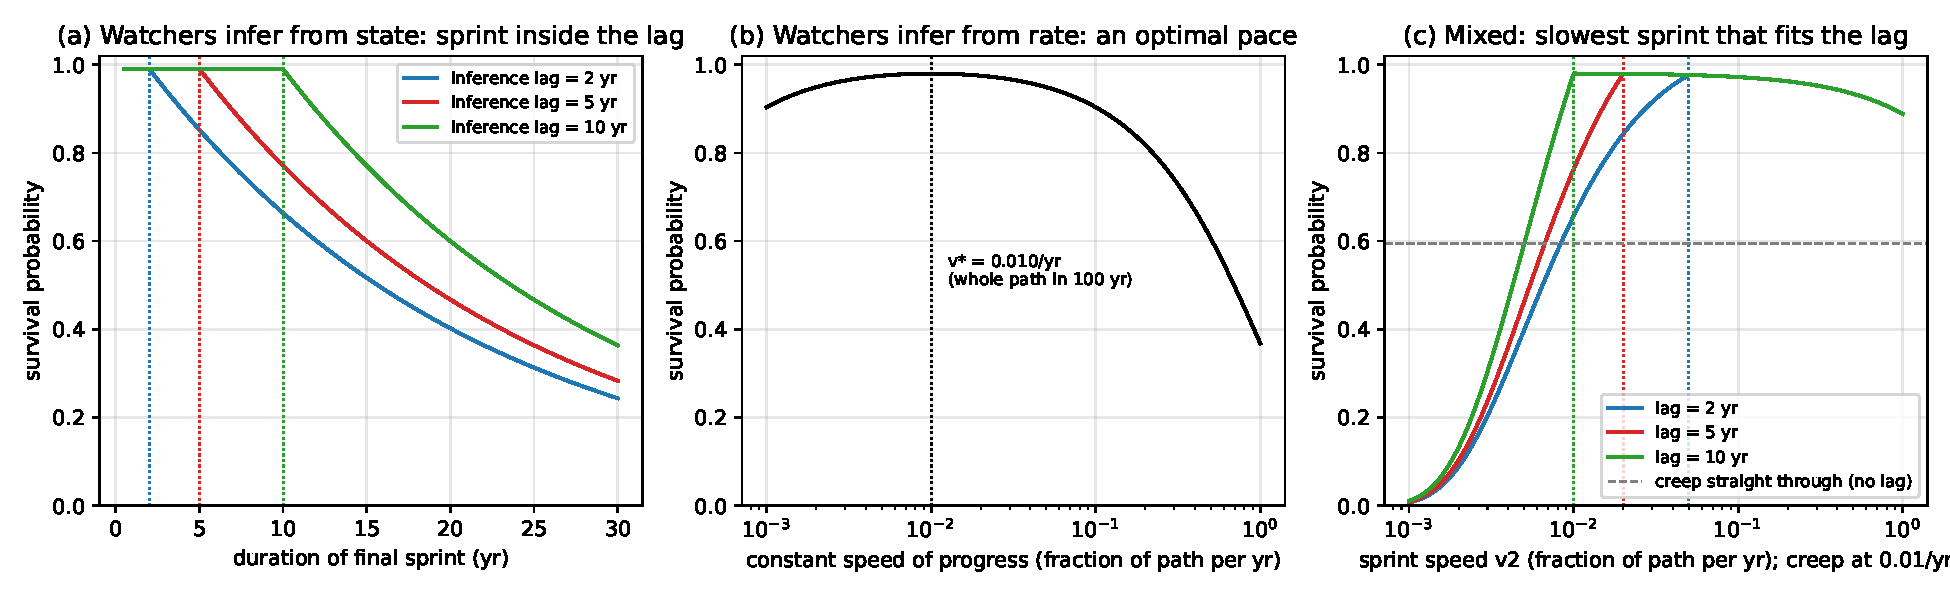
\includegraphics[width=\textwidth]{fig_pacing}
\caption{The pacing problem under illustrative parameters ($x_c = 0.9$; $h_0 = 10^{-4}$, $h_1 = 0.05$ per year; $h_2 = 1$ year; creep speed 0.01 of the path per year). (a) State regime: survival against the duration of the final sprint, for three inference lags; a sprint inside the lag is free. (b) Rate regime: survival against a constant speed of progress; the optimum $v^{*} = \sqrt{h_0/h_2}$ balances background hazard against visibility. (c) Mixed regime: survival against sprint speed for a fixed creep; the slowest sprint that fits the lag is optimal, and creeping straight through the danger zone (dashed) costs forty percent. Code with the paper.}
\label{fig:pacing}
\end{figure}

Two caveats attach, and the second is a finding. The creep-then-sprint policy is observationally indistinguishable from an ordinary logistic adoption curve, slow then fast then saturating, which any technological transition produces with no strategy behind it. Neither the civilization nor a watcher can infer intent from the shape of the curve, so the policy carries no signature of its own; this is a limitation of the result and also a small protection, since a watcher cannot read a sprint as a decision. And humanity's own trajectory, half a century of slow movement after 1972 followed by an abrupt acceleration in the last decade, matches the timing of the optimal policy and violates its other condition entirely: the sprint is supposed to occur inside the watchers' inference lag, unseen until done, and ours is the most visible thing the species has ever done. If the model is right, we are executing the timing of the best policy with the concealment of the worst.

\subsection{Planetary defence: the two halves of the paradox}
\label{sec:defence}

Deflecting asteroids is the single most effective natural-hazard measure a planet-bound civilization can take, and it bears on the strike procedure of Section~\ref{sec:strike} in two distinct ways that should not be confused.

The survey half is gain on two dimensions that should be kept apart, the natural and the artificial. A quiet delivery requires a poorly tracked body, because the target's only defence after the keyhole is to have the astrometry to recompute that body's orbit. Every improvement in completeness, from Rubin and from a dedicated infrared surveyor \citep{Jones2018,Mainzer2023}, shrinks the set of bodies a quiet delivery can use. Beyond some completeness no quiet delivery exists, and a strike must be loud: a large, late push visible to every rival. The link from the target's detection to the lineage's exposure should be made explicit, since they are different things: the target detecting a tracked body does not identify the lineage, but it forces the lineage either to abort, losing the delivery, or to deliver by a louder channel, a larger and later push or a different weapon, and it is the loud act that rivals can attribute. Completeness does not expose the lineage; it removes the quiet option and so raises the exposure cost $K$ of acting at all, and in the volunteer's dilemma a higher $K$ means more restraint. Two caveats attach. The attacker can substitute channels, so the claim is that completeness raises the cost of the cheapest channel rather than that it closes all of them. And a complete survey tells the watchers how good the target's prediction has become, which advances their estimate of its progress; we expect the protective effect to dominate, since it acts on payoffs while the signalling effect acts only on timing, but it is not guaranteed. Surveys do not merely let the civilization deflect; they make striking it more exposing for the strikers. In the natural-hazard dimension a complete survey is positive in every branch, including those in which there is no lurker hazard to reduce. In the lurker dimension it is protective wherever the quiet channel was the cheapest and the signalling effect is small, which we expect but cannot guarantee, and it does nothing against a hazard that is already absent, as in H2 and in fail-safe H3. It is the best argument for funding near-Earth-object surveys that has nothing to do with lurkers, and the one option in Table~\ref{tab:decision} whose natural-hazard value alone justifies it.

The display half is the paradox. Demonstrating deflection against a natural target shows a watcher that the civilization can do the one thing the watcher itself does, and advances the watcher's estimate of the civilization's progress. In H2 and H3 the display is harmless. In H4 it may read as T2 approaching. In H1 it brings the end of the window forward in the watchers' eyes. The resolution is to distinguish latent capability from demonstrated capability: hold the means to deflect, and the surveys that make them usable, without rehearsing them against natural targets more than once. The irony that the measure protects against exactly the weapon the model predicts is not lost on the authors of the model.

\subsection{Dual use, not pretence}
\label{sec:dualuse}

It is tempting to ask whether a civilization could pretend: broadcast loudly, look clumsy, and send apparently innocent missions past the belt carrying surveillance payloads. The model's answer is that it cannot, because the watcher reads everything the civilization publishes, including the argument that it should pretend. Intent cannot be concealed by a civilization that writes its intentions down. What can be concealed is capability, latent rather than demonstrated, as above. The coherent policy is therefore not pretence but genuine dual use: asteroid science that is also surveillance, deflection capability that is also deterrence, done for real reasons, so that there is no single intent for a watcher to infer. The civilization's first act of concealment, if it had wanted one, would have been not writing this paper.

Dual use has a second virtue that the companion paper's game makes precise. Watchers that can forecast a civilization's capabilities may still be unable to agree on its intentions. A replicating manufacturing programme built for settlement reads as T1 to a lineage that regards all replication as rivalry and as harmless to one that distinguishes defensive from expansionist replication. Where lineages disagree about whether an act is a trigger, only those that read it as one are potential strikers. It is tempting to conclude that fewer strikers means more safety, and the first draft of this paper did; the companion paper's game says otherwise. Let $n$ lineages be resident, $a$ of them reading the act as a trigger, and $d$ of them willing to punish an attacker they can locate, whether or not they read the act as a trigger. The strikers play the volunteer's dilemma among themselves with exposure cost $K(d) = V[1 - (1-\delta)^{d}]$, and survival is
\begin{equation}
Q(a,d) =
\begin{cases}
1, & K(d) \geq B,\\
\left(K(d)/B\right)^{a/(a-1)}, & K(d) < B,\ a \geq 2,\\
0, & K(d) < B,\ a = 1,
\end{cases}
\end{equation}
the first case because no one strikes when exposure exceeds benefit, the second the symmetric mixed equilibrium of the companion paper, the third a lone striker undeterred (Figure~\ref{fig:interp}). The form assumes that each punisher independently detects and acts with probability $\delta$; punishers whose capabilities or beliefs are correlated, or who form a coalition, count for less than their number, so $d$ should be read as the number of effectively independent punishers. Reducing $a$ at fixed $d$ \emph{lowers} survival, because diffusion of responsibility weakens, and reducing it to one is fatal unless the punishers alone deter. Interpretive heterogeneity protects only through $d$: it is protective where enough lineages would punish an attack they themselves did not consider justified, and harmful where they would not, since it then concentrates the decision in the least tolerant lineage with no rival to wait for. The civilization can cultivate ambiguity, by making its acts genuinely dual-purpose rather than by pretending, but the cultivation pays only in a crowded system whose lineages punish unjustified strikes, which is the regime in which the companion paper's protection already operates. The alignment drift of Section~\ref{sec:alignment} produces lineages that interpret differently; whether that is protective depends on how many of them would punish, which the third paper must settle.

\begin{figure}[!htbp]
\centering
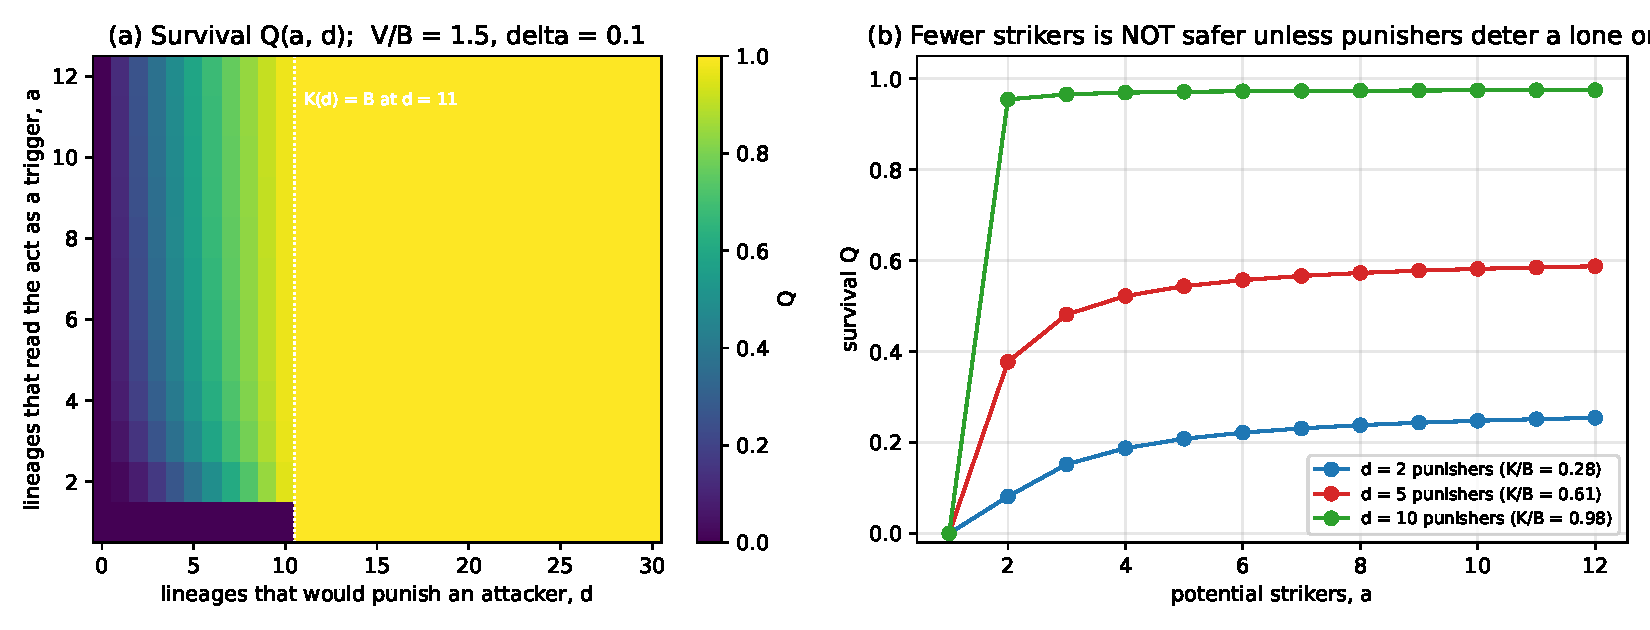
\includegraphics[width=\textwidth]{fig_interpretation}
\caption{Interpretive heterogeneity in the volunteer's dilemma, for $V/B = 1.5$ and per-punisher detection $\delta = 0.1$. (a) Survival $Q$ against the number of lineages that read the act as a trigger, $a$, and the number that would punish an attacker, $d$; the dotted line marks $K(d) = B$, beyond which a lone striker is deterred. (b) Sections at fixed $d$: fewer strikers is not safer unless the punishers alone deter a lone one. Code with the paper.}
\label{fig:interp}
\end{figure}

%% ---------------------------------------------------------------
\section{Where humanity stands}
\label{sec:window}

The companion paper defines the window's end as the acquisition of credible retaliation capacity \citep{Korhonen2013}, and three milestones that are often run together should be separated. The first is surviving a single planetary catastrophe, which a self-sufficient off-world population achieves. The second is technological reconstitution, rebuilding industry without Earth. The third is credible deterrence against an intelligent attacker, and it is defined by the expected cost the civilization can impose, not by its ability to hit an identified object. Against a resident probe network, a complete catalogue of the system's small bodies and the means to strike a located object, the survey-and-deflection capability of Section~\ref{sec:defence}, give local defence; they give deterrence only if what can be located and destroyed is a meaningful fraction of the lineage's local stake $V$, which destroying one expendable package is not. Credible retaliation therefore requires the ability to find the lineage's observers, not its shooters, and that is a harder problem than deflection. The third milestone does not follow from the first two and need not come after them, but it is further off than a catalogue. Which milestone the watchers count as T2 is unknown, and the dates below are scenarios for the first two. A lunar or Martian base dependent on Earth closes none of the three. Table~\ref{tab:milestones} sets humanity's milestones against the triggers they approach.

\begin{table}[!htbp]
\centering
\caption{Humanity's milestones against the triggers of Section~\ref{sec:threat}. ``Estimate'' is the watchers' estimate of progress toward the end of the window, as the model reads it.}
\label{tab:milestones}
\small
\begin{tabularx}{\textwidth}{@{}lXl@{}}
\toprule
Milestone & What a watcher reads & Trigger approached \\
\midrule
Broadcast radio, 1930s & Detectable technology; estimate begins & None \\
Industrial gases, 20th century & Persistent technosignature; enters the ghost-atmosphere census & None \\
Fission, 1945 & Weapons capability; estimate advances & None \\
Orbit, 1957; Moon, 1969 & Access to space; estimate advances & None \\
Deflection demonstrated, 2022 & Target can deflect; delivery must be covert and late & Display half of T2 \\
Crewed lunar return, 2020s & Not dispersal; dependent base & Slight \\
Heavy reusable launch, 2020s & Visible acceleration of the sprint & Rate signal \\
Capable artificial minds, 2020s & Ambiguous: kin or rival & T4 \\
Self-sufficient off-world settlement & First milestone, survival; the window closes only with the ability to find and punish & T2 (in part) \\
Catalogue plus deflection & Local defence and an early component of deterrence; not retaliation by itself & T2 (display half) \\
Locating the observer network & Ability to threaten a meaningful fraction of a lineage's local stake; the deterrence milestone & T2, T3 \\
Replicating manufacturing in space & Rival lineage in prospect & T1 \\
Interstellar launch & Rival lineage & T1, T2 \\
\bottomrule
\end{tabularx}
\end{table}

Three observations follow. First, humanity is late in its window by the model's reckoning and early by its own: ninety years detectable, no self-sufficient settlement, and the milestones that matter still ahead. Our estimate, offered as judgement informed by the literature rather than as a result, runs as follows. Genetic viability is the easy part and is well studied: Moore's early estimate of about 150 founders for a multigenerational voyage was revised upward by Smith to 14,000--44,000 once realistic mortality and disease were included \citep{Smith2014}, while Salotti's time-budget model finds that 110 settlers suffice for survival on Mars given full use of local resources and ideal organization \citep{Salotti2020}. Industrial self-sufficiency, the ability to rebuild the technology base, including semiconductor fabrication, without Earth, is a far stricter condition; we know of no published estimate of the population it requires, and the breadth of a modern supply chain suggests a settlement of order $10^{5}$--$10^{6}$ people, a judgement rather than a result. It is the second milestone, not the third: a settlement that could survive Earth's loss removes the attacker's certainty of a clean kill but does not by itself impose a cost on the attacker, so it does not establish deterrence. Metzger and colleagues argue that a self-expanding lunar industry could be bootstrapped from about twelve tonnes of landed equipment in about twenty years \citep{Metzger2013}, which is the fastest route on paper, and it runs through self-replicating manufacturing, which is T1. Life-support closure on the International Space Station remains partial, with water recovery above ninety percent and oxygen recovery about half, and an independent assessment of the one settlement plan that claimed near-term independence found that its resource assumptions failed \citep{Do2016}. Current programmes put a crewed lunar base in the 2030s and a crewed Mars landing in the late 2030s or 2040s \citep{NASA2024}, both dependent on Earth; the one organization that states self-sufficiency as its goal has not published a date with engineering behind it. On any current path, then, Earth-independence arrives no earlier than about 2100, and plausibly between 2100 and 2200. That places the end of humanity's window 75 to 175 years ahead, and its total length, from detectability in the 1930s, at roughly 170 to 270 years, which agrees with the companion paper's $10^{2}$--$10^{3}$ yr and with the 200-yr median that Sandberg and Armstrong assumed independently \citep{SandbergArmstrong2013}. The watchers' estimate may run ahead of this, because replicating manufacturing in space, T1, is likely to precede self-sufficiency, T2, by decades. Second, the order in which the remaining milestones are being approached is, incidentally, the lower-trigger order. A Moon-first programme has ordinary explanations in cost and politics, and the model does not need a secret one; but a lunar base dependent on Earth does not close the window, whereas a self-sufficient Mars settlement does, so Moon first is also what approaching the threshold slowly and ambiguously would look like. A civilization behaving optimally and one behaving ordinarily look alike here, as they did for the pacing curve. The same is true of the programmes already in existence, kinetic deflection, infrared surveys, the Rubin survey, the asteroid missions: each has an ordinary justification, and the model's claim is only that an awakening civilization would build the same list for its own reasons. Third, the unilateralist's curse applies within the civilization. The date at which humanity crosses T1 is set not by its governments but by the least restrained actor able to launch a replicator, and the model turns Forgan's observation about the futility of moratoria \citep{Forgan2019} into a hazard with a mechanism.

%% ---------------------------------------------------------------
\section{A surveillance programme for the home system}
\label{sec:surveillance}

The awakening civilization can learn its branch, and can detect a strike in preparation, with observations it is making anyway, provided it knows what the model says to look for. What follows are candidate discriminants, not validated tests: none has a known sensitivity or specificity, each needs a physically realistic null model before a detection could be called surprising, and the distinction between finding a suspicious configuration and computing how surprising it is under that null is the whole of the statistical work still to be done.

\paragraph{What the visits so far tell us} Spacecraft have visited about a dozen asteroids, out of more than a million larger than a kilometre: a sampling of one in a hundred thousand, and a biased one, since missions go to what is scientifically interesting or cheap to reach, the largest bodies and the near-Earth objects, which is exactly the set a lineage avoids. None of those missions read as a search, and none crossed a trigger. They establish that no detectable lurker sits on or near the surface of those dozen bodies at the resolution achieved, and nothing about the rest. The first informative visit will be to a body chosen for the properties a lurker would want rather than for the ones a planetary scientist wants, and that mission should be thought about carefully before it flies.

\paragraph{Acceleration anomalies and their false positives} Surveys detect Yarkovsky accelerations near $2 \times 10^{-13}$~m/s$^2$ on well-tracked bodies \citep{Greenberg2020}, and a keyhole push of a micrometre per second applied years ahead lies at that scale, so the act of delivery is not detectable as an anomaly. Larger pushes are, and there the model must contend with a known natural class: the dark comets, small inactive near-Earth objects with non-gravitational accelerations of order $10^{-10}$~au/d$^{2}$, far above Yarkovsky, nonradial, with no detected coma, attributed to seasonal outgassing on rapidly rotating bodies \citep{Seligman2023,Taylor2023}. They are the false-positive population for any acceleration criterion, and a candidate must be separated from them: their accelerations are sustained and modulated by heliocentric distance and rotation, whereas a push is transient, and the criteria of Section~\ref{sec:iso}, non-inverse-square, impulsive, post-anomaly trajectory toward a resonance, are what separate the two. The expected false-positive rate is set by the dark-comet population, which Rubin will characterize.

\paragraph{Keyhole statistics, the primary test} Because the push is undetectable, the test is its consequence. The procedure predicts an excess of poorly observed near-Earth objects on trajectories that pass through keyholes, relative to what a dynamical model of the population with its selection effects produces. That null model must be built explicitly, since resonance trapping, dynamical diffusion and incomplete orbits all place bodies near keyholes naturally, and the discriminating observation is then a body found inside a keyhole corridor whose prior astrometry, reanalysed, is better fitted with a small impulse than without one. Impact solutions removed by later astrometry are mostly orbit-determination error; the few that are not would show the same signature. Nobody has examined either population with this question in mind. The next step requires no evidence of probes at all: a numerical null model that propagates a realistic near-Earth population through known dynamics and survey selection, yields the distribution of natural keyhole passages, and asks whether a hypothesized micrometre-per-second intervention would be distinguishable in simulated astrometry. That calculation would be a reproducible result whatever the truth of the hypothesis, and it is the one we would do first.

\paragraph{Architecture as a predictor} Because delivery latency and quiet-strike availability both depend on the supply of near-miss bodies, suppression should correlate with system architecture: scarred ghosts more common, and dispersed survivors rarer, in systems with an asteroid belt stirred by a giant planet. This sharpens the companion paper's population test and exposes a subtlety in its design. Matching controls on debris-disk properties removes the natural impact-rate difference, but the artificial excess scales with debris availability too, so matching partly removes the signal. The statistic should be an interaction: on technosignature worlds the impact rate rises faster with debris than it does on controls. The lurker signal is in the difference of slopes, not of levels.

\paragraph{Orbital families with no parent} A belt interferometer is many small dark bodies with correlated orbits. In the Rubin catalogue it would appear as an orbital family that cannot have formed by collision. Family-finding algorithms search for collisional parents; a search for families without one has not been run.

\paragraph{Derelicts, by structure} Branches H2 and H3 are identifiable from the home system: wreckage of two or more lineages with dynamical scars, or a single weathered derelict. Candidate locations are Earth's co-orbital population \citep{Benford2019}, where Kamo`oalewa's lunar-like spectrum \citep{Sharkey2021} is the natural cover a lineage would choose, the Lagrange regions \citep{HaqqMisraKopparapu2012}, the lunar surface \citep{DaviesWagner2013,Ellery2025}, and Jupiter's Trojans \citep{Levison2021}. Section~\ref{sec:rock} predicts that lurker hardware is built from local material, so spectroscopy will not find it; the discriminants are structural, geometry, internal voids, thermal inertia and radar polarization inconsistent with a rubble pile or a monolith.

\paragraph{Radar, the active edge} Planetary radar has pinged thousands of asteroids for decades. It is active, but a ping that returns a normal signature reveals nothing to either side, and routine radar is part of ordinary astronomy. The risky step remains rendezvous with a specific suspicious object, and the ordering is: passive surveys first; radar on candidates that passive data flag; rendezvous only against objects whose passive signature already suggests a derelict rather than a functioning node, since a derelict cannot be triggered.

\paragraph{The hazard of looking, weighed} T3 makes searching risky in one branch and, as Section~\ref{sec:threat} argued, less risky than it first appears. Not searching leaves the civilization blind to a nudge in progress and unable to learn its branch. The ordering above resolves it.

\paragraph{A note on unidentified aerial phenomena} The model predicts that lurkers are never seen as craft near the target. The lineage's entire strategy is concealment, close sentinels are kept few and dark, and a machine manoeuvring near the target's aircraft would be the loudest possible violation of it. If such reports described real machines, they would be evidence against the model's agents, not for them.

%% ---------------------------------------------------------------
\section{Villages in the forest}
\label{sec:villages}

The companion paper argued that cooperation among lineages is rare, because an ally's mistake exposes both and the ally cannot be vetted, and that where it exists it is among kin sharing codes fixed before launch. Section~\ref{sec:rock} found the one exception: physical proximity, where mutual vulnerability enforces a truce and a private channel exists. Whether a truce formed on a rock persists off it is open, but the mechanism is clear, and it is the same one that applies to civilizations. A civilization's own colonies share its history and values. Neighbouring systems a few light-years apart can exchange signals within a lifetime, so for them the repeated game that light-lag otherwise destroys is restored. And probes make interaction local and verifiable. The cooperative form the forest permits is therefore the hidden enclave: kin and near neighbours communicating by tight beam, invisible from outside, visible only to an observer on the line between two stars. For an awakening civilization this sets the shape of any expansion it undertakes, as a quiet network of kin rather than a visible frontier, and it predicts one observable for the exoplanet programme, optical leakage along aligned pairs of stars.

%% ---------------------------------------------------------------
\section{What to do, and what to expect}
\label{sec:recommend}

The analysis above reduces to a short list, and the list has a property that matters more than any single item on it: every recommendation is something a prudent civilization would do without believing the model, so that if there are no lurkers nothing has been lost. Table~\ref{tab:recommend} gives each action, its effect by branch, the observable consequence the model predicts, and when that consequence could be seen.

\begin{table}[!htbp]
\centering
\caption{Recommendations, their effect, and what the model predicts will follow.}
\label{tab:recommend}
\footnotesize
\begin{tabularx}{\textwidth}{@{}>{\raggedright\arraybackslash}p{3.1cm}>{\raggedright\arraybackslash}p{2.6cm}>{\raggedright\arraybackslash}X>{\raggedright\arraybackslash}p{1.9cm}@{}}
\toprule
Action & Effect by branch & Predicted observable & When \\
\midrule
Complete the near-Earth-object survey to small sizes & Reduces natural hazard in all branches; raises every lineage's $K$ where the quiet channel was cheapest & Under lurkers: an excess of poorly observed bodies in keyhole corridors whose prior astrometry fits better with a small impulse; larger thrust-like accelerations separated from the dark-comet population. Under none: Yarkovsky, dark comets and orbit error only & 2030s \\
Bind visibly on self-replicating machines & Lowers $B$; raises $Q$ in H1; defers T1 in H4 & None directly; the one near-term trigger we control is taken off the table & Now \\
Do not transmit & Neutral or better in all branches & None & Now \\
No replicators before dispersal; seed them after & Avoids T1; after the window, the companion paper's recommended move & None & Mid-century decision \\
Hold deflection capability, do not rehearse & Avoids advancing a confirmer's estimate; neutral against forecasters & None & Now \\
Moon first; Mars built as a switch & Helps against confirmers; neutral against forecasters; free & None & 2030s--2100 \\
Passive search in order; pre-register interstellar criteria & Identifies the branch without T3 & Wreckage (H2), one structural derelict (H3), nothing (H1, H4); interstellar population natural or with a patrol fraction & 2030s \\
Do not remove a found node & Preserves the standoff in H1 & If removed in H1: hazard jumps to the least restrained remaining lineage & Contingent \\
Keep publishing & Pretence impossible; dual use is the policy & None & Ongoing \\
Artificial minds & Sign unknowable (T4) & None & Ongoing \\
\bottomrule
\end{tabularx}
\end{table}

Three predictions summarize the table. If the civilization does all of this and lurkers exist, nothing visible happens for decades, and the hazard is concentrated at the approach to self-sufficiency, after 2100 on current paths, with replicating manufacturing in space as the one trigger likely to arrive earlier. If it rushes instead, a single visible push to independence, early replicators, deliberate messaging, then under an untriggered lurker with a replicator trigger a keyhole nudge follows within years of the launch, which a complete survey would see in time; under a crowded system the dilemma is played at the window's end with survival of order $K/B$; under the dead branches, nothing. And if there are no lurkers, the civilization ends with a complete asteroid catalogue, a governance regime for its own replicators, a careful settlement architecture, and no messages sent. The recommendations are low-regret rather than regret-free, and the costs should be named: a moratorium on transmission forgoes whatever contact might have offered, restraint on replicators and on visible expansion delays capabilities a civilization may want for other reasons, and surveys and settlement architectures cost money. The claim is that caution remains rational while those costs are modest relative to a terminal downside, which is the only kind of claim a conditional theory is entitled to make.

%% ---------------------------------------------------------------
\section{Notes on the companion paper}
\label{sec:errata}

Working out the threat model has turned up five points at which the companion paper \citep{Lopin2026} should be read with a correction or a qualification. We record them here rather than leave them for a referee.
\begin{enumerate}
  \item \emph{T3 is weaker than stated.} Under a design that separates observers from shooters, detection of a node exposes that node only. T3 is a kill trigger only if detection credibly leads to the lineage's whole local presence being removed (Section~\ref{sec:threat}).
  \item \emph{Branch H3 is safe only under fail-safe design.} A shooter package built to act unless told not to is triggered by its observer's decay (Section~\ref{sec:strike}). The companion paper's hazard table should split H3 accordingly.
  \item \emph{Lineages can coordinate on shared rocks.} The companion paper assumes no coordination because communication exposes the sender. Two packages on one body share a private channel and a mutual hostage, and coalitions formed there reduce the effective number of players (Section~\ref{sec:rock}). The sign of the net effect on $Q$ is open.
  \item \emph{Berserker galaxies are dark.} The companion paper's discussion of galaxy-scale infrared nulls treats a conquered galaxy as a bright one. Free probe replication consumes belts, not starlight; the null constrains loud surviving civilizations, not monocultures (Section~\ref{sec:berserker}).
  \item \emph{Matching controls on debris removes part of the signal.} The artificial impact excess scales with the supply of near-miss bodies, as the natural rate does, so the population test should use the interaction, the slope of impact rate against debris on technosignature worlds relative to controls, rather than the level difference (Section~\ref{sec:surveillance}).
\end{enumerate}
None of these changes the companion paper's conditional claims; the first and fourth strengthen them, the second and third qualify a branch and an assumption, and the fifth sharpens a test.

%% ---------------------------------------------------------------
\section{Conclusions}
\label{sec:conclusions}

Conditional on the companion paper's premises, an awakening civilization can conclude the following about its situation and its conduct.
\begin{enumerate}
  \item Resident lurkers act at the last decisive moment, through a pipeline rather than a command: a body pre-positioned by resonance drift onto a near-miss orbit, a push of micrometres per second years before a close approach, passage through a gravitational keyhole, impact on a resonant return years later, mop-up by a second package, and a shooter consumed at impact; the decision falls at the last steer opportunity before the window closes, a stopping time set by orbital geometry as much as by the target. The lineage stays. Its choice among autonomous, confirm-to-act and keep-alive architectures determines whether the defunct-lurker branch is safe; only keep-alive makes it dangerous, and selection works against keep-alive.
  \item Two lineages on one rock are each other's hostages; where their thresholds are close they form the first coalition rather than fighting, and boarded rocks are both the most dangerous objects in the system and the only place rivals can speak. Lurker hardware is forensically anonymous, and there is no quiet-and-brief delivery.
  \item Earth's record contains no evidence of a strike, and one indication against: Chicxulub has no mop-up tail. On Earth a reset rescheduled intelligence rather than preventing it; whether that generalizes is unknown. Of the interstellar objects, one fits part of a patrol signature and none fits a delivery; criteria for the next are stated in advance.
  \item Three decisions minimize lurker hazard in every branch within the model, assuming no offsetting benefits: observe passively, do not transmit, do not launch replicators before dispersal. A fourth, completing the near-Earth-object survey, reduces natural hazard in every branch and lurker hazard wherever a quiet delivery was the cheapest option, because it forces any strike to be loud and so raises every lurker's exposure cost. Interpretive heterogeneity among the watchers protects only where enough of them would punish an unjustified strike.
  \item Two dilemmas remain. The pacing of dispersal, where against watchers who confirm the optimal policy creeps and then crosses the last interval inside their lag, but where against watchers who forecast from a gigayear of cases there is no lag, and the remaining levers are the payoffs: raise $K$ by completing the surveys, lower $B$ by binding visibly on replicators. And the display of deflection capability, resolved by holding the means without rehearsing them.
  \item A surveillance programme that costs nothing in trigger terms can both identify the branch and detect a strike in preparation: refined acceleration criteria, keyhole statistics, parentless orbital families, structural rather than spectral derelict searches, and passive before active.
\end{enumerate}
The central tension restated: safety from nature and safety from watchers pull apart, and the civilization's task is to find the path on which they pull least. The model's answer is that the two coincide more often than the paradox suggests, since the surveys that protect against natural impacts are the same surveys that make artificial ones expensive, and that the places they diverge, display and visible dispersal, are exactly the places where restraint costs the civilization nothing it needs.

\section*{Data availability}
No observational data were used. The code for Figures~\ref{fig:pacing} and~\ref{fig:interp} is released with the paper.

\section*{Declaration of generative AI and AI-assisted technologies in the writing process}
During the preparation of this work the author used Claude (Anthropic) to develop and stress-test the argument in dialogue and to draft the manuscript. The author reviewed and edited the content and takes full responsibility for it.

%% ---------------------------------------------------------------
\begin{thebibliography}{99}

\bibitem{Lopin2026} L. Lopin, Lurker ecology: rival embedded probes and a falsifiable resolution of the Fermi paradox, SSRN preprint 7668018 (2026).

\bibitem{Dam2026} H. Dam, First attack, final offensive: the dark forest on an open roster, arXiv:2609.12003 (2026).

\bibitem{Korhonen2013} J.M. Korhonen, MAD with aliens? Interstellar deterrence and its implications, Acta Astronaut. 86 (2013) 201--210.

\bibitem{JebariAsker2024} K. Jebari, A.S. Asker, Saved by the dark forest: how a multitude of extraterrestrial civilizations can prevent a Hobbesian trap, The Monist 107 (2024) 176--189.

\bibitem{SandbergArmstrong2013} A. Sandberg, S. Armstrong, Hunters in the dark: game theory analysis of the deadly probes scenario, poster, National Astronomy Meeting (NAM2013), St Andrews, 2013.

\bibitem{Brin2014} G.D. Brin, The search for extraterrestrial intelligence (SETI) and whether to send `messages' (METI): a case for conversation, patience and due diligence, J. Br. Interplanet. Soc. 67 (2014) 8--16.

\bibitem{Bostrom2016} N. Bostrom, T. Douglas, A. Sandberg, The unilateralist's curse and the case for a principle of conformity, Soc. Epistemol. 30 (2016) 350--371.

\bibitem{Forgan2019} D.H. Forgan, Predator--prey behaviour in self-replicating interstellar probes, Int. J. Astrobiol. 18 (2019) 552--561.

\bibitem{Hrdy2009} S.B. Hrdy, Mothers and Others: The Evolutionary Origins of Mutual Understanding, Harvard University Press, Cambridge, MA, 2009.

\bibitem{Daly2023} R.T. Daly, et al., Successful kinetic impact into an asteroid for planetary defence, Nature 616 (2023) 443--447.

\bibitem{BailerJones2018} C.A.L. Bailer-Jones, J. Rybizki, R. Andrae, M. Fouesneau, New stellar encounters discovered in the second Gaia data release, Astron. Astrophys. 616 (2018) A37.

\bibitem{FischerGodde2024} M. Fischer-G\"odde, J. Tusch, S. Goderis, et al., Ruthenium isotopes show the Chicxulub impactor was a carbonaceous-type asteroid, Science 385 (2024) 752--756.

\bibitem{Pickersgill2021} A.E. Pickersgill, D.F. Mark, M.R. Lee, et al., The Boltysh impact structure: an early Danian impact event during recovery from the K--Pg mass extinction, Sci. Adv. 7 (2021) eabe6530. 

\bibitem{Kyte1998} F.T. Kyte, A meteorite from the Cretaceous/Tertiary boundary, Nature 396 (1998) 237--239.

\bibitem{TuryshevToth2017} S.G. Turyshev, V.T. Toth, Diffraction of electromagnetic waves in the gravitational field of the Sun, Phys. Rev. D 96 (2017) 024008.

\bibitem{Ruddiman2003} W.F. Ruddiman, The anthropogenic greenhouse era began thousands of years ago, Clim. Change 61 (2003) 261--293.

\bibitem{Valsecchi2003} G.B. Valsecchi, A. Milani, G.F. Gronchi, S.R. Chesley, Resonant returns to close approaches: analytical theory, Astron. Astrophys. 408 (2003) 1179--1196.

\bibitem{Chesley2006} S.R. Chesley, Potential impact detection for near-Earth asteroids: the case of 99942 Apophis (2004 MN$_4$), Proc. IAU Symp. 229 (2006) 215--228. 

\bibitem{Micheli2018} M. Micheli, D. Farnocchia, K.J. Meech, et al., Non-gravitational acceleration in the trajectory of 1I/2017 U1 (`Oumuamua), Nature 559 (2018) 223--226.

\bibitem{BialyLoeb2018} S. Bialy, A. Loeb, Could solar radiation pressure explain `Oumuamua's peculiar acceleration?, Astrophys. J. Lett. 868 (2018) L1.

\bibitem{BergnerSeligman2023} J.B. Bergner, D.Z. Seligman, Acceleration of 1I/`Oumuamua from radiolytically produced H$_2$ in H$_2$O ice, Nature 615 (2023) 610--613.

\bibitem{DeschJackson2021} S.J. Desch, A.P. Jackson, 1I/`Oumuamua as an N$_2$ ice fragment of an exo-Pluto surface II, J. Geophys. Res. Planets 126 (2021) e2020JE006807.

\bibitem{Loeb2025} A. Loeb, Anomalies of 3I/ATLAS, organized by likelihood, online essay (2025). %% [web source; replace with any peer-reviewed version before submission]

\bibitem{Manfroid2021} J. Manfroid, D. Hutsem\'ekers, E. Jehin, Iron and nickel atoms in cometary atmospheres even far from the Sun, Nature 593 (2021) 372--374.

\bibitem{Ivezic2019} \v{Z}. Ivezi\'c, S.M. Kahn, J.A. Tyson, et al., LSST: from science drivers to reference design and anticipated data products, Astrophys. J. 873 (2019) 111.

\bibitem{Jones2018} R.L. Jones, C.T. Slater, J. Moeyens, et al., The Large Synoptic Survey Telescope as a near-Earth object discovery machine, Icarus 303 (2018) 181--202.

\bibitem{Mainzer2023} A. Mainzer, et al., The Near-Earth Object Surveyor mission, Planet. Sci. J. 4 (2023) 224. 

\bibitem{Seligman2023} D.Z. Seligman, D. Farnocchia, M. Micheli, et al., Dark comets? Unexpectedly large nongravitational accelerations on a sample of small asteroids, Planet. Sci. J. 4 (2023) 35.

\bibitem{Taylor2023} A.G. Taylor, D. Farnocchia, D. Vokrouhl\'ick\'y, D.Z. Seligman, J.K. Steckloff, M. Micheli, Seasonally varying outgassing as an explanation for dark comet accelerations, Icarus 408 (2024) 115822.

\bibitem{Wiegert2024} P. Wiegert, On the sensitivity of Apophis' 2029 Earth approach to small asteroid impacts, Planet. Sci. J. 5 (2024) 184.

\bibitem{Greenberg2020} A.H. Greenberg, J.-L. Margot, A.K. Verma, P.A. Taylor, S.E. Hodge, Yarkovsky drift detections for 247 near-Earth asteroids, Astron. J. 159 (2020) 92.

\bibitem{Griffith2015} R.L. Griffith, J.T. Wright, J. Maldonado, M.S. Povich, S. Sigur{\dh}sson, B. Mullan, The $\hat{G}$ infrared search for extraterrestrial civilizations with large energy supplies. III, Astrophys. J. Suppl. Ser. 217 (2015) 25.

\bibitem{Benford2019} J. Benford, Looking for lurkers: co-orbiters as SETI observables, Astron. J. 158 (2019) 150.

\bibitem{Sharkey2021} B.N.L. Sharkey, V. Reddy, R. Malhotra, et al., Lunar-like silicate material forms the Earth quasi-satellite (469219) 2016 HO3 Kamo`oalewa, Commun. Earth Environ. 2 (2021) 231.

\bibitem{HaqqMisraKopparapu2012} J. Haqq-Misra, R.K. Kopparapu, On the likelihood of non-terrestrial artifacts in the Solar System, Acta Astronaut. 72 (2012) 15--20.

\bibitem{DaviesWagner2013} P.C.W. Davies, R.V. Wagner, Searching for alien artifacts on the Moon, Acta Astronaut. 89 (2013) 261--265.

\bibitem{Ellery2025} A. Ellery, Technosignatures of self-replicating probes in the Solar System, arXiv:2510.00082 (2025).

\bibitem{Smith2014} C.M. Smith, Estimation of a genetically viable population for multigenerational interstellar voyaging: review and data for Project Hyperion, Acta Astronaut. 97 (2014) 16--29.

\bibitem{Salotti2020} J.-M. Salotti, Minimum number of settlers for survival on another planet, Sci. Rep. 10 (2020) 9700.

\bibitem{Metzger2013} P.T. Metzger, A. Muscatello, R.P. Mueller, J. Mantovani, Affordable, rapid bootstrapping of the space industry and solar system civilization, J. Aerosp. Eng. 26 (2013) 18--29.

\bibitem{Do2016} S. Do, A. Owens, K. Ho, S. Schreiner, O. de Weck, An independent assessment of the technical feasibility of the Mars One mission plan, Acta Astronaut. 120 (2016) 192--228.

\bibitem{NASA2024} NASA, Moon to Mars Architecture Definition Document (ESDMD-001), NASA, Washington, DC, 2023, and subsequent annual revisions.

\bibitem{Levison2021} H.F. Levison, C.B. Olkin, K.S. Noll, et al., Lucy mission to the Trojan asteroids: science goals, Planet. Sci. J. 2 (2021) 171.

\end{thebibliography}

\end{document}
